\documentclass[a4paper, 10pt]{article}
\usepackage[margin = 1in]{geometry}
\usepackage{amsmath}
\usepackage{tabularx}
\usepackage{framed}
\setlength{\parindent}{0em}
\newcolumntype{L}{>{\arraybackslash}m{10cm}}
\newcolumntype{T}{>{\arraybackslash}m{6cm}}
\usepackage{graphicx}
\usepackage{pdfpages}

\begin{document}

\section*{Topic 11 - Wave Motion}
\begin{framed}
   A \textbf{progressive wave} is one that transfers energy from one point to another in the direction of wave propagation
\end{framed}	
\begin{itemize}
   \item particles oscillate about their equilibrium positon
\end{itemize}	

\section{Wave terminology}
\begin{itemize}
   \item \textbf{Displacement} of a particle is the distance travelled in a specific direction from its equilibrium position
   \item \textbf{Amplitude, A} of a wave is the magnitude of maximum displacement of a particle from eqm position
   \item \textbf{Period, T} of a wave is the time taken for a particle to complete one oscillation 
   \item \textbf{Frequency, F} is the numebr of oscillations per unit tiem made by a particle of a wave, \[
   T = \frac{1}{f}
   \]
\item \textbf{Wavelength $\lambda$} is the distance between two consecutive points which are in phase
\item \textbf{Speed, v} is the distance travelled by a wave per unit time
   \[
   v = \lambda f = \frac{\lambda}{T}
   \]
   
\item \textbf{Phase / Phase angle, $\phi$ } is a measure of the fraction of a cylce that has been completed by an on oscillating particle or by a wave. 
\item \textbf{Phase difference} between two partciles in a wave or between two waves at a point is the measure of the fraction of a cycle which one is ahead of the other
   \begin{itemize}
      \item \textbf{In phase}: particles exercute the same motion at the same time, $\phi = 0$ 
      \item \textbf{Out of phase}: partciles that are at different stages of motion
      \item \textbf{Anti-phase}: execute motions that are out of phase by $\pi$ rad 
   \end{itemize}	
\item \textbf{Wavefront} is a line or surface joining points on a wave that are in phase. Wave travels in a direction perpendicular to the wavefront
\end{itemize}	

\subsection{graphs of waves}
\begin{minipage}{0.5\textwidth}
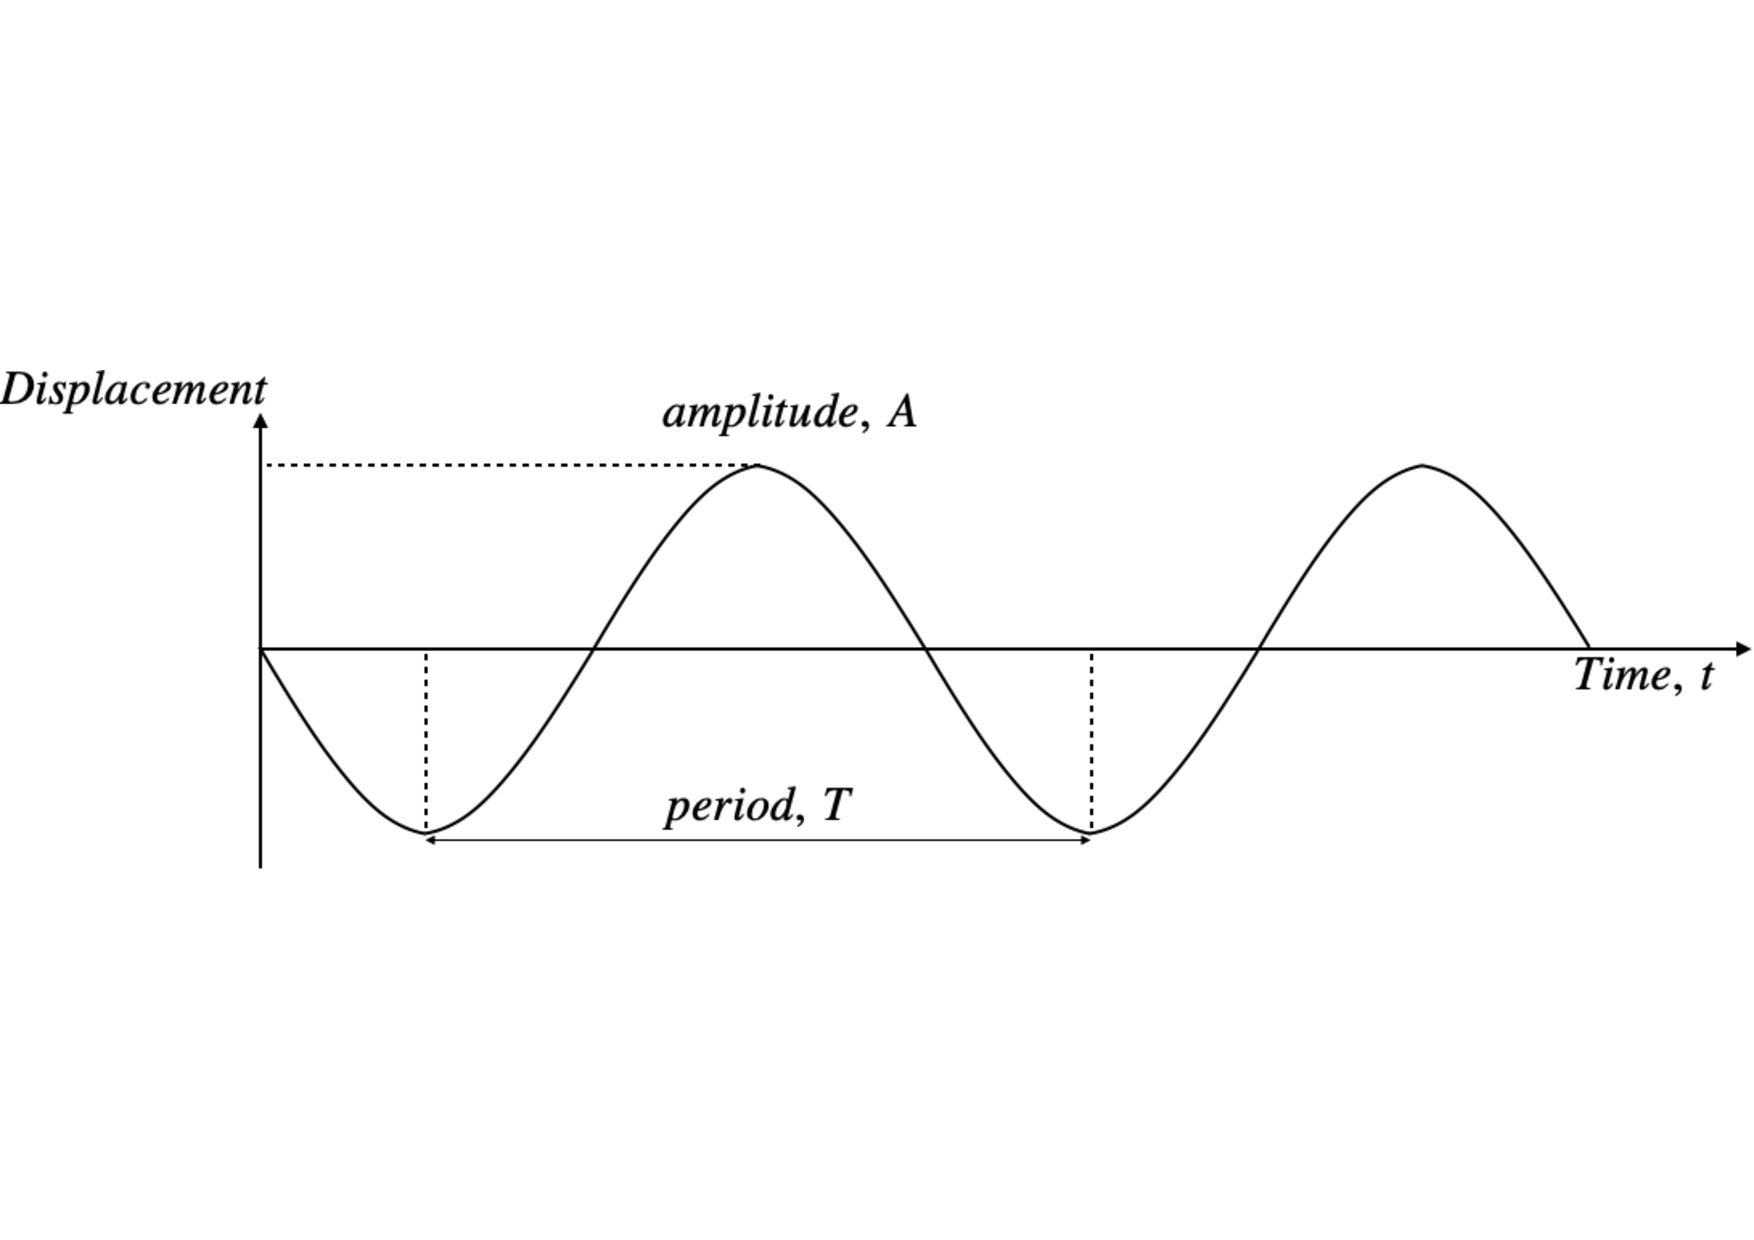
\includegraphics[trim = 50 50 50 50, width=6cm]{figures/1.pdf}
\end{minipage}	
\begin{minipage}{0.5\textwidth}
\textbf{Displacemennt - time graph} \\
graph represents displacement of \textbf{one} particle over time 
\end{minipage}	
\begin{minipage}{0.5\textwidth}
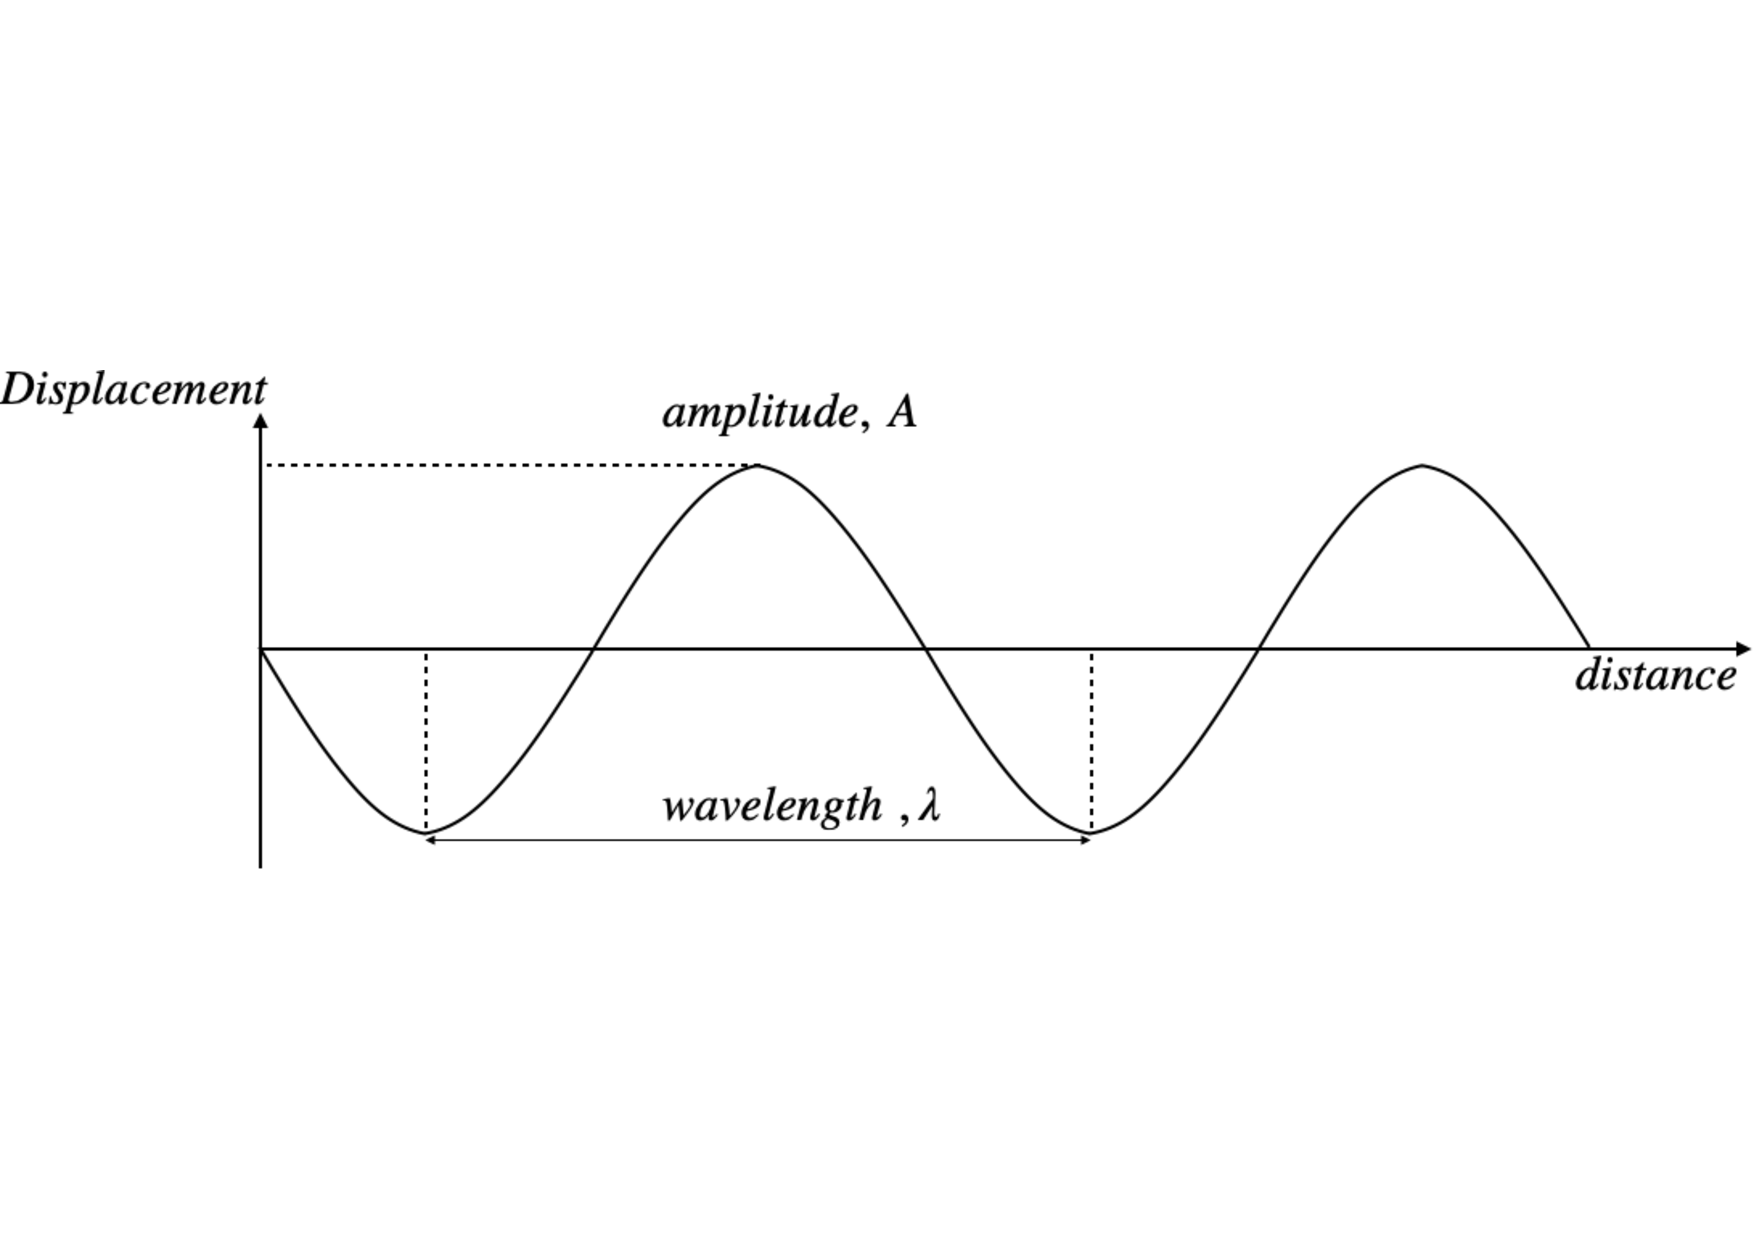
\includegraphics[trim = 50 50 50 50, width=6cm]{figures/2.pdf}
\end{minipage}	
\begin{minipage}{0.5\textwidth}
   \textbf{Displacement - distance graph} \\
graph represents the displacement of \textbf{all} particles at a particular instant
\end{minipage}	


\subsection{representation of phase difference}
For a wave travelling to the right \\
\begin{minipage}{0.5\textwidth}
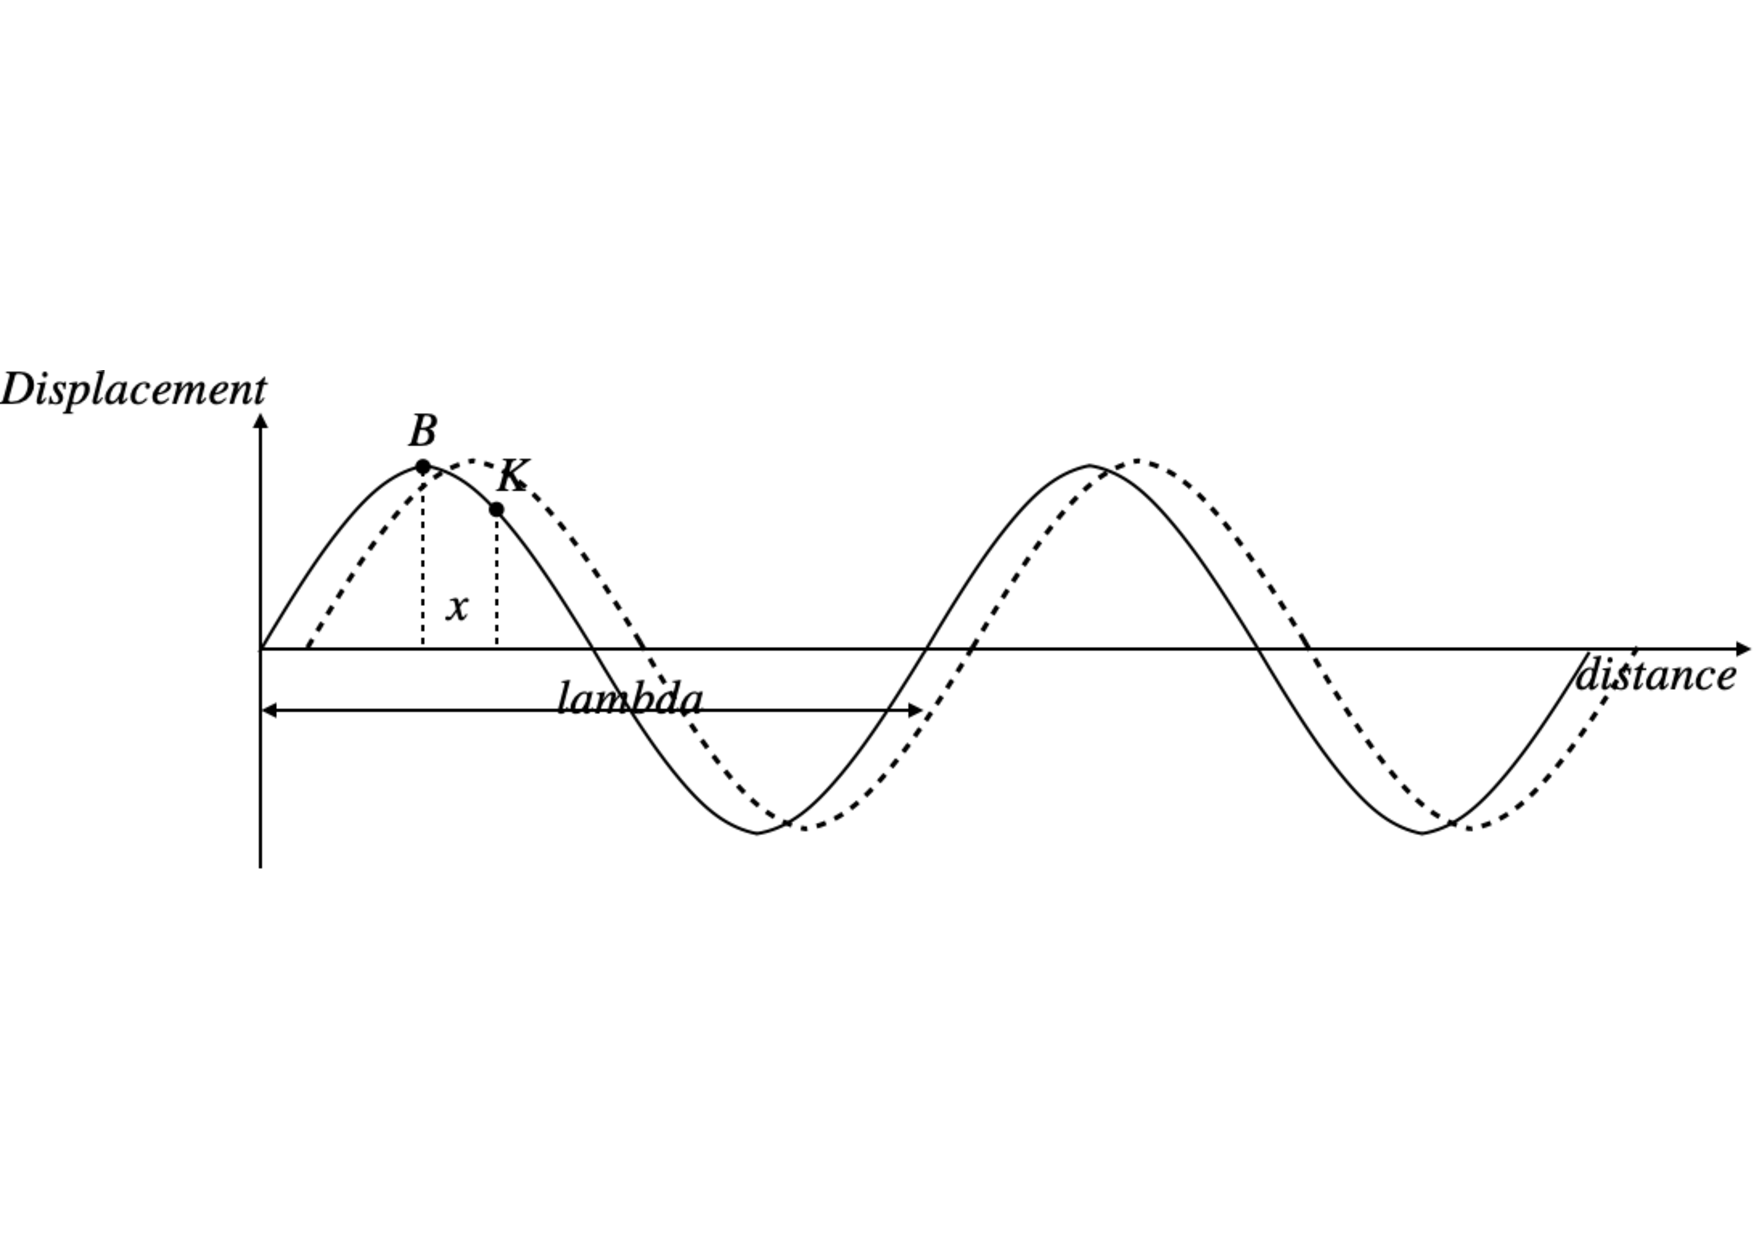
\includegraphics[trim = 50 50 50 50, width=6cm]{figures/3.pdf}
\end{minipage}	
\begin{minipage}{0.5\textwidth}
\textbf{Displacemennt - distance graph} \\
   B is on its way down and K is on its way up \\
   K is lagging B by a phase differene of $\phi$ or (B is ahead of K by $\phi$), $0 \le \phi \pi$ 
   \[
   \frac{x}{\lambda} = \frac{\phi}{2\pi}
   \]
   \[
   \phi = 2 \pi \frac{x}{\lambda}
   \]
\end{minipage}	

\begin{minipage}{0.5\textwidth}
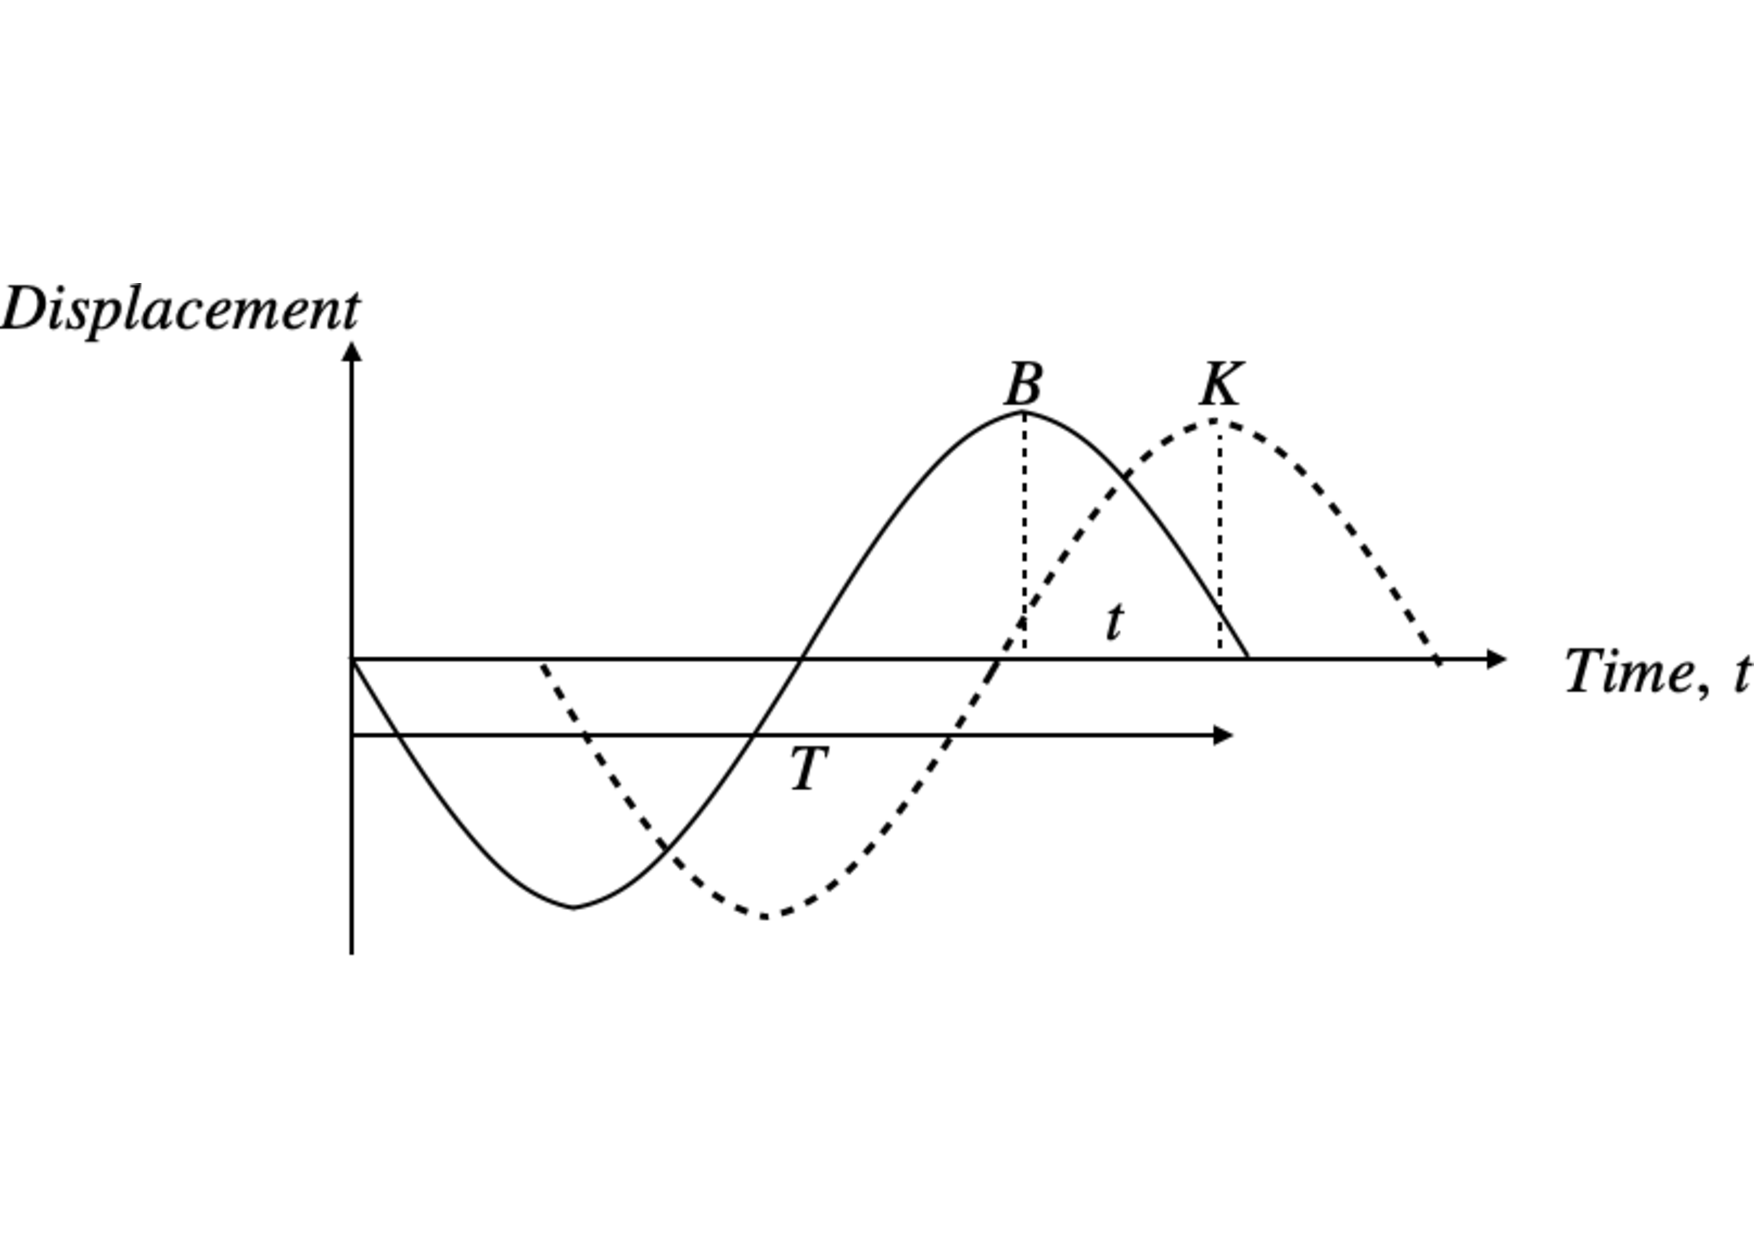
\includegraphics[trim = 50 50 50 50, width=6cm]{figures/4.pdf}
\end{minipage}	
\begin{minipage}{0.5\textwidth}
\textbf{Displacemennt - time graph} \\
   K is lagging B by a phase differene of $\phi$ or (B is ahead of K by $\phi$), $0 \le \phi \pi$   
   \[
   \frac{t}{T} = \frac{\phi}{2\pi}
   \]
   \[
   \phi = 2 \pi \frac{t}{T}
   \]
\end{minipage}	

\section{Wave Intensity}
\begin{framed}
   The \textbf{intensity} of a wave is defined as the rate of transfer of energy per unit area, where the area measured is perpendicular to the direction of energy transfer
   \[
   I = \frac{P}{S}
   \]
where $P$ is the power of the source, and $S$ is the surface area of the wave front
\[
I = kA^2
\]
\end{framed}	

\subsection{Point source and inverse square}
for a point source emitting waves that spread out radially, with a spherical wavefront, the further away from the source, the larger the area where energy is being distributed \\
\begin{minipage}{0.5\textwidth}
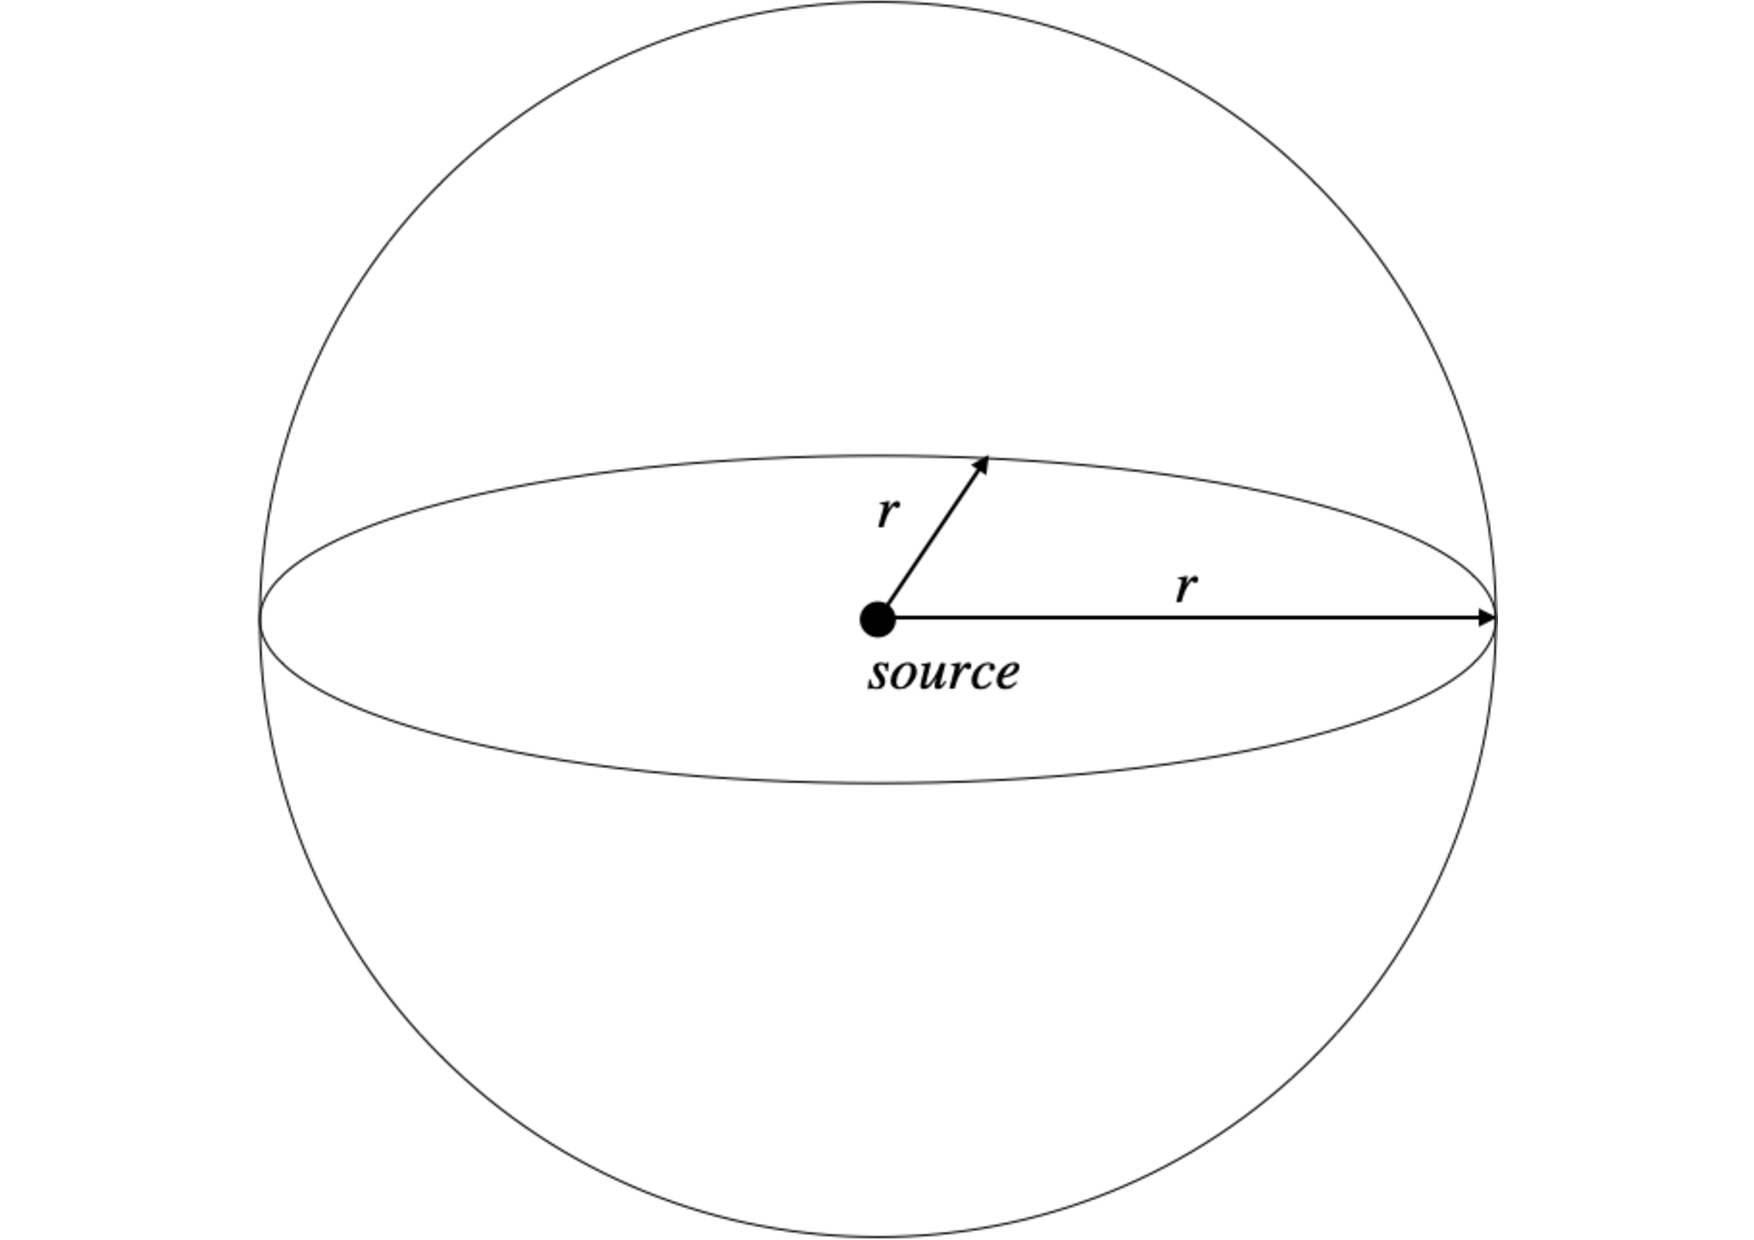
\includegraphics[trim = 50 50 50 50, width=4cm]{figures/5.pdf} 
\end{minipage}	
\begin{minipage}{0.5\textwidth}
\[
I = \frac{P}{4\pi r^2}
\]

Hence for a constant power, the inverse square law is known as 
\[
I = \frac{k}{r^2}
\]
\end{minipage}	

\section{Transverse and longitudinal waves}
\begin{framed}
   A \textbf{transverse wave} is one in which particles oscillate in a direction perpendicular to the direction of energy transfer \\

   A \textbf{longitudinal wave} is one in which the particles oscillate in a direction parallel to the direction of energy transfer
\end{framed}	

\subsection{EM waves}
Important properties
\begin{itemize}
   \item Do not require medium to propagate, can move through vacuum
   \item EM waves travel at a speed of $c = 3.00 \times 10^8 ms^{-1}$ in vacuum
   \item EM waves are transverse waves and can hence be polarised
\end{itemize}	
\begin{center}
   \begin{tabular}{c | c | c | c | c | c | c | c}
      Radiation type & Radio & Microwave & Infrared & Visible & Ultraviolet & X-ray & Gamma ray \\
      \hline
      Wavelength (m) & $10^3$ & $10^{-2}$ & $10^{-5}$ & $0.5 \times 10^{-6}$ & $10^{-8}$ & $10^{-10}$ & $10^{-12}$  \\
      Frequency(Hz) & $10^4$  & $10^8$ & $10^{12}$ & $10^{15}$ & $10^{16}$ & $1o^{18}$ & $10^{20}$ 

   \end{tabular}
\end{center}

\subsection{Sound waves}
\begin{itemize}
   \item \textbf{compression}: regions where particles are compressed together, regions of high pressure
   \item \textbf{rarefraction}: regions where particles are spread apart, regions of low pressure
\end{itemize}	

\section{polarisation}
\begin{framed}
   \textbf{Polarisation} is a phenomenon where the oscillations of the wave particles in a transverse wave are restricted to one direction only and this direction is perpendicular to the direction of wae propagation or energy transfer
   \begin{itemize}
      \item hence does not apply to longitudinal waves
   \end{itemize}	
\end{framed}	

\subsection{Intensity}
When unpolarised light is incident on an ideal polariser, 
\[
I = \frac{I_0}{2}
\]

\subsection{Malus' Law}
\begin{framed}
   \textbf{Malus' Law} states that the intensity of a beam of plane polarised light after passing through a plane polariser varies with the square of the cosine of the angle through which the polariser is rotated from the position that gives maximum intensity
   \[
   I = I_0 cos^2 \theta
   \]
   
\end{framed}	


When plane polarised light passes through a second polariser with its polarising axis at an angle of $\theta$ from the first polariser, the resultant amplitude is
\[
 A = A_0 cos\theta
\]
Since 
\begin{align*}
   I &= kA^2 \\
     &= k(A_0 cos\theta)^2 \\
     &= kA_0^2 cos^2 \theta \\
     &= I_0 cos^2 \theta
\end{align*}	


\end{document}	

